\subsection{Proactive Headcount and Suspicious Activity Detection using YOLOv8}

\subsubsection{Resumen}
Este estudio aborda la creciente necesidad de monitoreo de multitudes en espacios públicos debido al aumento de la población mundial. Utiliza un sistema de inteligencia artificial para la detección proactiva de actividades sospechosas y el conteo de personas en tiempo real mediante el modelo de detección de objetos YOLOv8. El objetivo principal es mejorar la seguridad en entornos con alta densidad de personas, detectando incidentes como la presencia de armas, fuego, caídas y humo.

\subsubsection{Metodología}
El modelo emplea el algoritmo YOLOv8 para la detección de objetos en tiempo real, proporcionando evaluaciones instantáneas de la densidad de multitudes y detectando actividades anómalas. Se utilizó una base de datos que contiene aproximadamente 500 imágenes distribuidas en diferentes clases (personas, armas, fuego, humo, etc.), procesadas en la plataforma Roboflow para aumentar su precisión y robustez.

\begin{figure}[h] % "h" indica que la imagen se coloque aproximadamente aquí
    \centering
    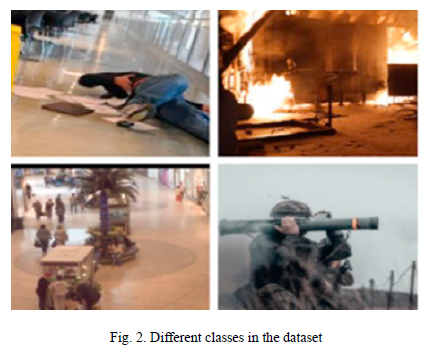
\includegraphics[width=0.6\textwidth]{4/met1.png} % Ruta y tamaño de la imagen
    \label{fig:ejemplo} % Etiqueta para referenciar la imagen
\end{figure}

\subsubsection{Procesamiento de Datos}
Los datos fueron preprocesados mediante técnicas de aumento como rotación, volteo y desenfoque, obteniendo un total de 1066 imágenes para el entrenamiento del modelo. Este proceso de preprocesamiento se realizó para asegurar la eficacia del modelo en diferentes condiciones ambientales.

\begin{figure}[h] % "h" indica que la imagen se coloque aproximadamente aquí
    \centering
    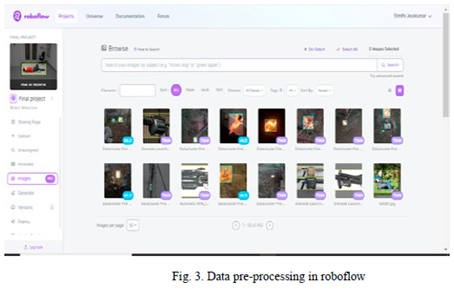
\includegraphics[width=0.6\textwidth]{4/pro1.png} % Ruta y tamaño de la imagen
    \label{fig:ejemplo} % Etiqueta para referenciar la imagen
\end{figure}

\subsubsection{Entrenamiento del Modelo}
El modelo YOLOv8 se seleccionó por su capacidad para evaluar densidades de multitudes y su rapidez en la detección de actividades anómalas. Se realizaron pruebas de rendimiento comparando diferentes versiones de YOLOv8, siendo YOLOv8n (versión nano) la que mejor equilibró precisión y velocidad para el análisis en tiempo real.

\begin{figure}[h] % "h" indica que la imagen se coloque aproximadamente aquí
    \centering
    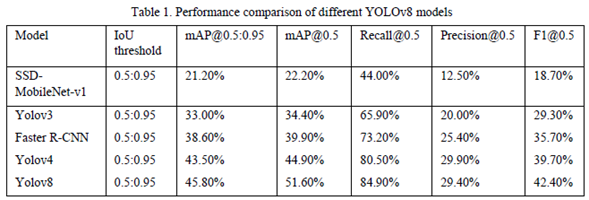
\includegraphics[width=0.8\textwidth]{4/tab1.1.png} % Ruta y tamaño de la imagen
    \label{fig:ejemplo} % Etiqueta para referenciar la imagen
\end{figure}

\begin{figure}[h] % "h" indica que la imagen se coloque aproximadamente aquí
    \centering
    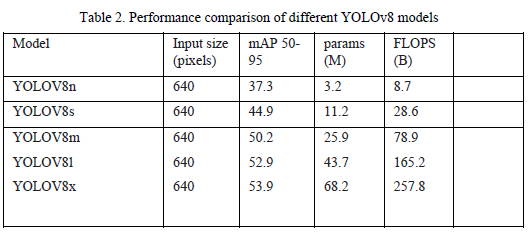
\includegraphics[width=0.8\textwidth]{4/tab1.2.png} % Ruta y tamaño de la imagen
    \label{fig:ejemplo} % Etiqueta para referenciar la imagen
\end{figure}

\begin{figure}[h] % "h" indica que la imagen se coloque aproximadamente aquí
    \centering
    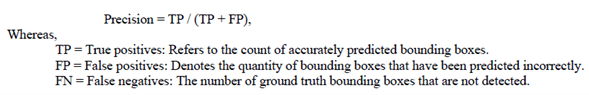
\includegraphics[width=0.8\textwidth]{4/tab1.3.png} % Ruta y tamaño de la imagen
    \label{fig:ejemplo} % Etiqueta para referenciar la imagen
\end{figure}

\begin{figure}[h] % "h" indica que la imagen se coloque aproximadamente aquí
    \centering
    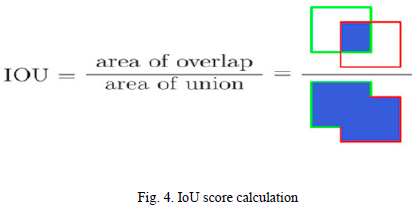
\includegraphics[width=0.8\textwidth]{4/tab1.4.png} % Ruta y tamaño de la imagen
    \label{fig:ejemplo} % Etiqueta para referenciar la imagen
\end{figure}

\clearpage

\subsubsection{Evaluación de Resultados}
El modelo alcanzó una precisión promedio superior al 95\% en la detección de actividades sospechosas y el conteo de personas en tiempo real. Este sistema permitió identificar actividades específicas como acceso no autorizado, merodeo y objetos desatendidos con alta precisión, enviando alertas instantáneas a los encargados de seguridad mediante Twilio.

\begin{figure}[h] % "h" indica que la imagen se coloque aproximadamente aquí
    \centering
    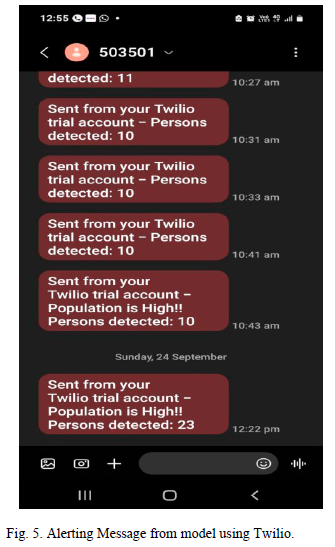
\includegraphics[width=0.6\textwidth]{4/re1.png} % Ruta y tamaño de la imagen
    \label{fig:ejemplo} % Etiqueta para referenciar la imagen
\end{figure}

\clearpage


\subsubsection{Limitaciones}
Algunas limitaciones del sistema incluyen la falta de pruebas en entornos no controlados, la dependencia de la calidad de las cámaras y posibles problemas de latencia en la transmisión de datos. Además, el sistema enfrenta desafíos en la generalización de su efectividad ante diversas culturas y eventos específicos.

\subsubsection{Conclusión y Aporte del Estudio}
La integración de YOLOv8 para la detección en tiempo real y el uso de Twilio para alertas instantáneas demuestran ser una solución poderosa para el monitoreo proactivo de seguridad. El estudio sugiere que para futuras investigaciones de este tipo nos enfoquemos en realizar pruebas en entornos variados y evaluar el impacto de la calidad de las cámaras en el rendimiento del sistema.



\subsection{Suspicious Activity Detection using LSTM and MobileNetV2}

\subsubsection{Resumen}
Este estudio explora la combinación de redes neuronales LSTM y MobileNetV2 para la detección de actividades sospechosas en secuencias de video. El objetivo principal es mejorar la capacidad de los sistemas de vigilancia para identificar patrones de movimiento sospechosos en tiempo real en entornos de alta densidad. La combinación de estos modelos permite capturar tanto la información temporal como espacial de los movimientos, mejorando así la precisión en la clasificación de actividades.

\subsubsection{Metodología}
La metodología del estudio se basa en la integración de redes LSTM (para la captura de dependencias temporales) y MobileNetV2 (para la clasificación visual en cada cuadro de video). La LSTM se encarga de analizar la secuencia de imágenes en el tiempo, permitiendo la detección de anomalías en patrones de movimiento, mientras que MobileNetV2 clasifica las características visuales de cada imagen, detectando objetos y posturas sospechosas.

\begin{figure}[h] % "h" indica que la imagen se coloque aproximadamente aquí
    \centering
    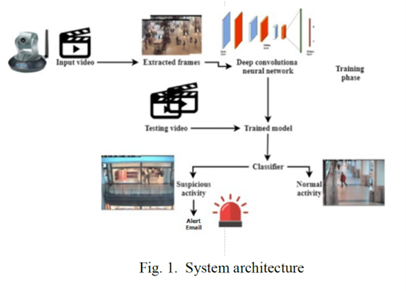
\includegraphics[width=1.0\textwidth]{4/met2.png} % Ruta y tamaño de la imagen
    \label{fig:ejemplo} % Etiqueta para referenciar la imagen
\end{figure}

\clearpage

\subsubsection{Procesamiento de Datos}
El estudio utiliza un conjunto de datos de video que incluye situaciones normales y sospechosas en áreas urbanas. Los datos fueron procesados para garantizar la precisión en la detección en tiempo real. La preprocesación de los datos incluyó técnicas de filtrado para reducir el ruido y mejorar la calidad de los cuadros, facilitando así la clasificación de actividades sospechosas.

\subsubsection{Entrenamiento del Modelo}
El modelo fue entrenado con el conjunto de datos preprocesado utilizando TensorFlow y Keras. La validación cruzada k-fold se empleó para optimizar el rendimiento y ajustar los hiperparámetros de ambas redes. Además, se utilizó RandomizedSearchCV para ajustar parámetros específicos de MobileNetV2 y LSTM, maximizando la precisión en la detección de actividades sospechosas en tiempo real.

\subsubsection{Evaluación de Resultados}
Los resultados mostraron una precisión del 88\% en la detección de actividades sospechosas, especialmente en la identificación de comportamientos como merodeo y movimientos repetitivos en áreas restringidas. Este enfoque demostró ser efectivo para la vigilancia en tiempo real, emitiendo alertas automáticas cuando se detectan patrones sospechosos.

\subsubsection{Limitaciones}
El estudio presenta algunas limitaciones, como la dificultad para generalizar los resultados en entornos no controlados y la sensibilidad a la calidad del video. La precisión del modelo depende en gran medida de la calidad de las imágenes, por lo que en condiciones de baja resolución la precisión podría verse afectada.

\subsubsection{Conclusión y Aporte del Estudio}
La integración de LSTM y MobileNetV2 para la detección en tiempo real de actividades sospechosas demostró ser una solución robusta en entornos urbanos. El estudio sugiere realizar pruebas adicionales en diversos entornos y explorar la posibilidad de mejorar la eficiencia mediante el ajuste fino de hiperparámetros para adaptarse a diferentes resoluciones de video.








\subsection{Toward Trustworthy Human Suspicious Activity Detection}

\subsubsection{Resumen}
Este estudio aborda la necesidad de confiabilidad en los sistemas de detección de actividades sospechosas, integrando un enfoque de evaluación de confianza para reducir falsas alarmas y aumentar la precisión en zonas urbanos. El objetivo es mejorar la precisión del sistema al identificar comportamientos sospechosos mientras se minimizan las alertas falsas, generando así un sistema de vigilancia más robusto y seguro.

\subsubsection{Metodología}
La metodología emplea una combinación de técnicas de detección de objetos y algoritmos de análisis de confianza para evaluar la probabilidad de que una actividad sea sospechosa. El sistema utiliza un modelo de aprendizaje profundo que combina redes convolucionales para el análisis de imágenes y algoritmos de evaluación de confianza para mejorar la precisión en la detección de actividades anómalas.

\begin{figure}[h] % "h" indica que la imagen se coloque aproximadamente aquí
    \centering
    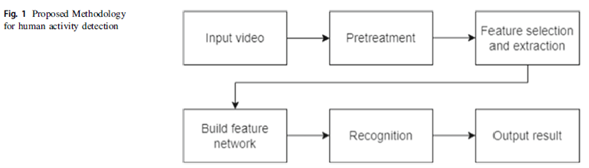
\includegraphics[width=0.8\textwidth]{4/met3.png} % Ruta y tamaño de la imagen
    \label{fig:ejemplo} % Etiqueta para referenciar la imagen
\end{figure}


\subsubsection{Procesamiento de Datos}
El sistema fue entrenado con un conjunto de datos de video que incluye situaciones variadas, desde actividades cotidianas hasta comportamientos potencialmente sospechosos. Para mejorar la precisión, el conjunto de datos fue preprocesado mediante técnicas de normalización de imágenes y reducción de ruido, lo que permitió optimizar la detección de actividades sospechosas en entornos de baja calidad de video.

\begin{figure}[h] % "h" indica que la imagen se coloque aproximadamente aquí
    \centering
    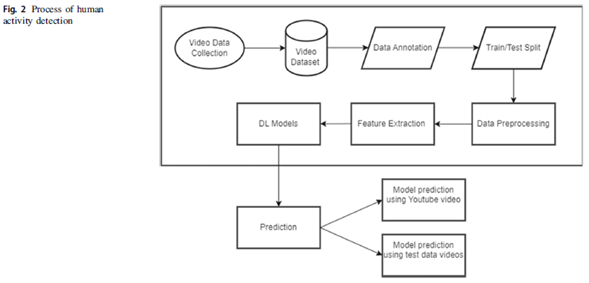
\includegraphics[width=0.8\textwidth]{4/pro3.png} % Ruta y tamaño de la imagen
    \label{fig:ejemplo} % Etiqueta para referenciar la imagen
\end{figure}



\subsubsection{Entrenamiento del Modelo}
Se utilizó Python y TensorFlow para entrenar el modelo de redes neuronales convolucionales (CNN) y el sistema de evaluación de confianza. El ajuste de hiperparámetros se realizó mediante validación cruzada y se optimizaron los parámetros de confianza para minimizar las falsas alarmas. Este enfoque permitió mejorar la confiabilidad del sistema en entornos urbanos.

\begin{figure}[h] % "h" indica que la imagen se coloque aproximadamente aquí
    \centering
    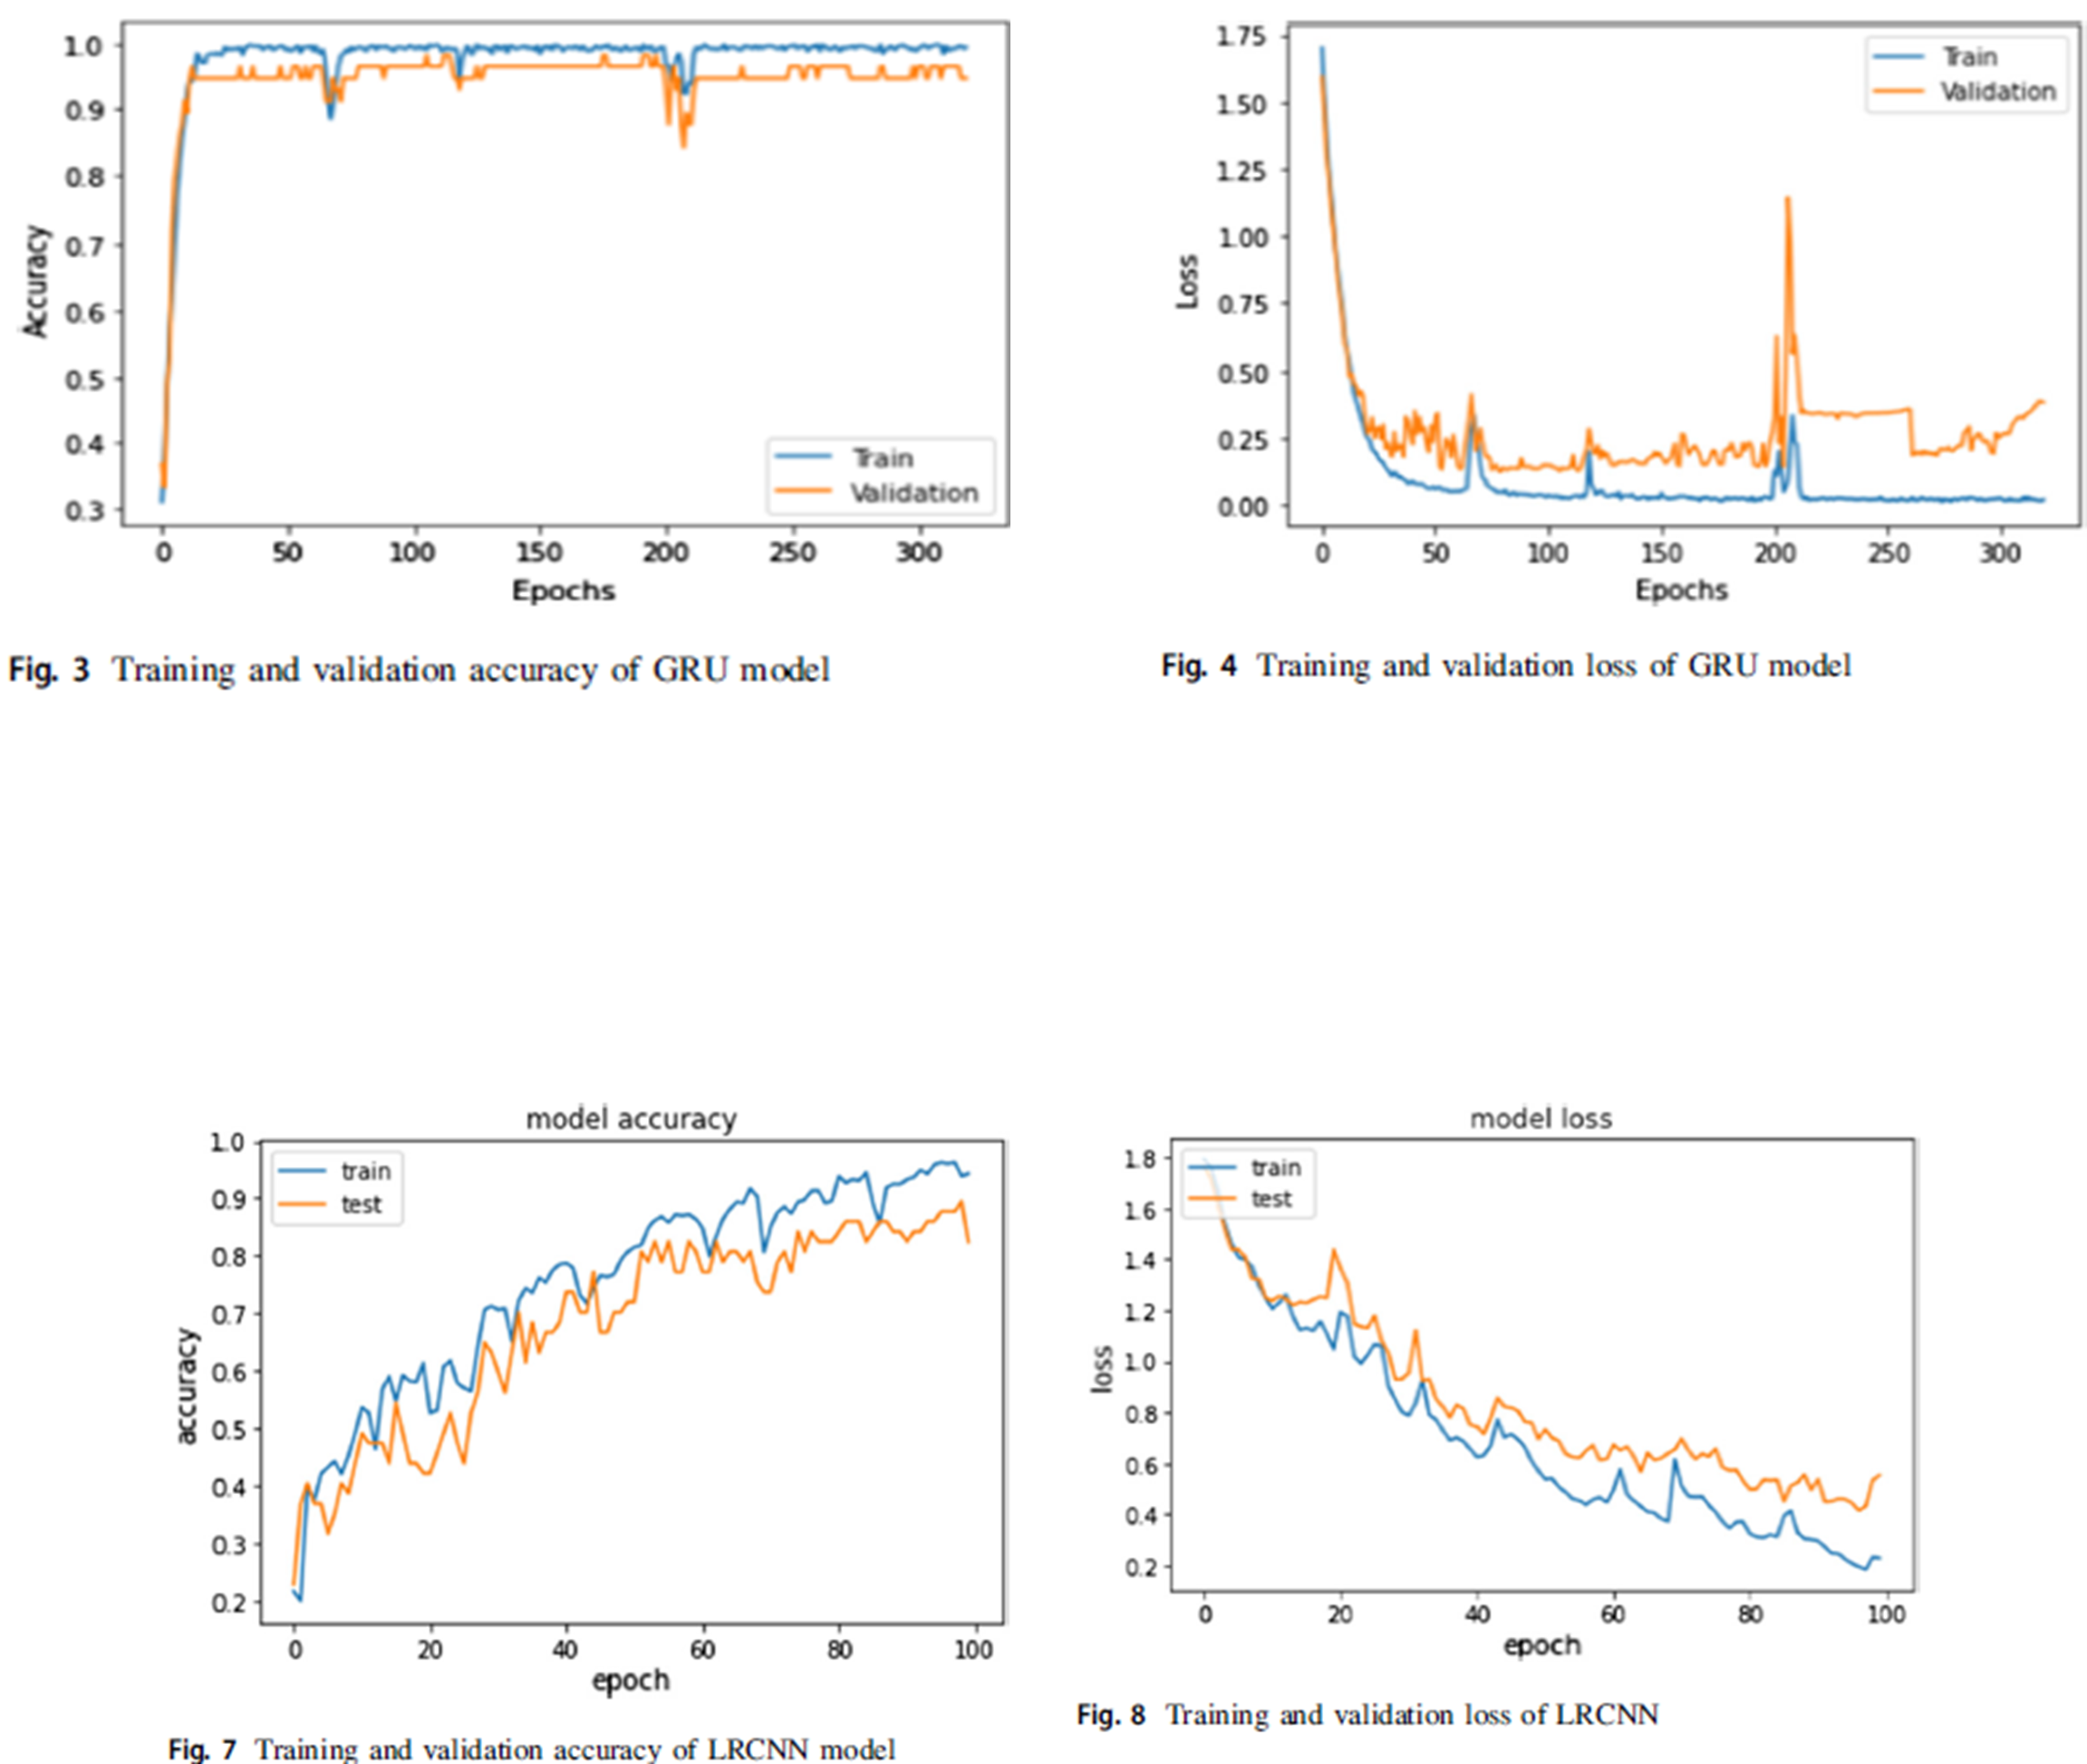
\includegraphics[width=1.1\textwidth]{4/entre 3.png} % Ruta y tamaño de la imagen
    \label{fig:ejemplo} % Etiqueta para referenciar la imagen
\end{figure}

\clearpage


\subsubsection{Evaluación de Resultados}
El sistema alcanzó una precisión del 91.55\% en la detección de actividades sospechosas, superando otros modelos tradicionales de detección en entornos urbanos. Además, el enfoque de evaluación de confianza permitió reducir las falsas alarmas en un 20\%, lo cual representa una mejora significativa en la confiabilidad del sistema para entornos de vigilancia.

\begin{figure}[h] % "h" indica que la imagen se coloque aproximadamente aquí
    \centering
    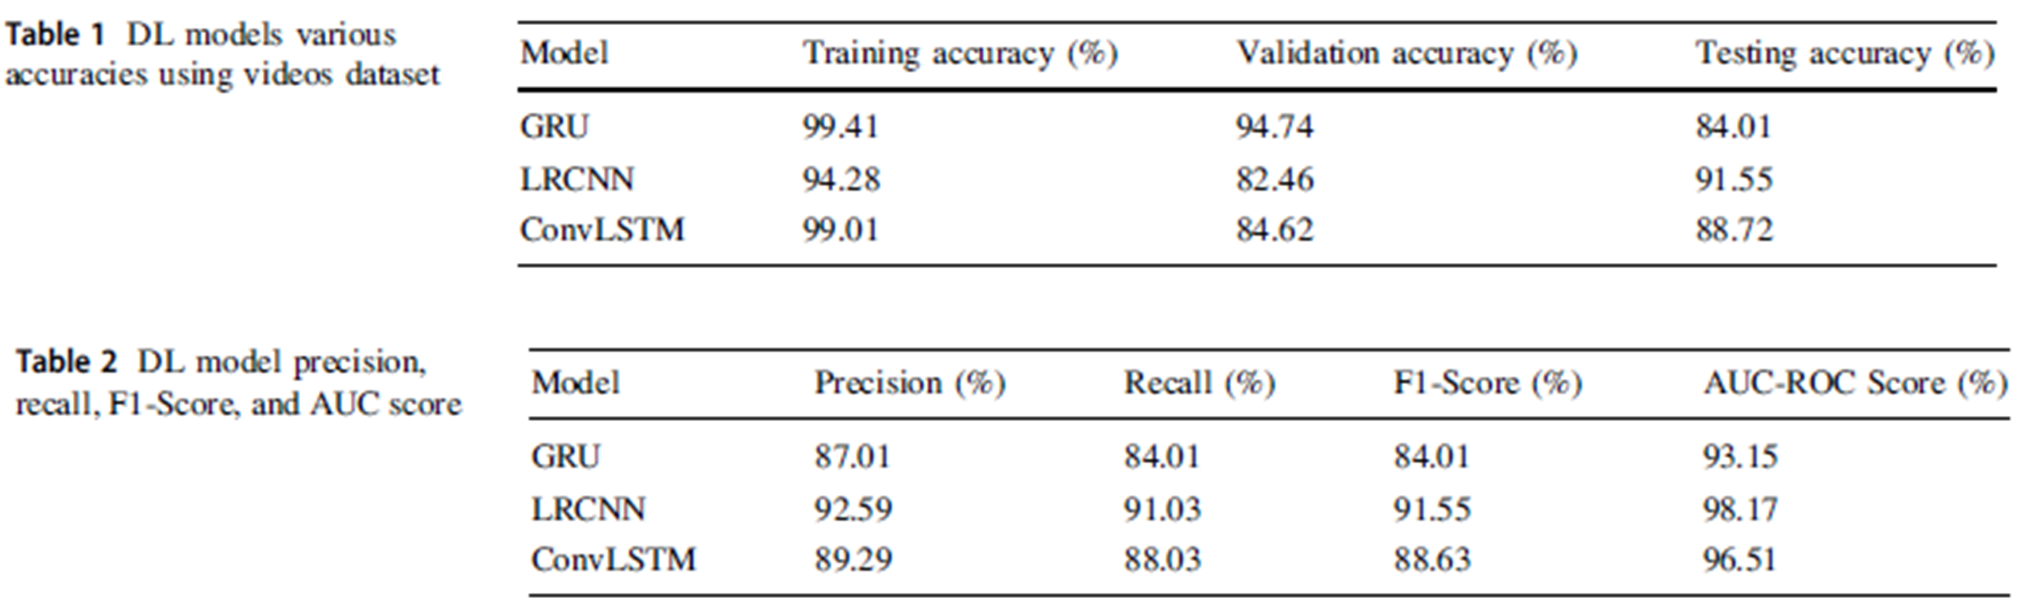
\includegraphics[width=1.0\textwidth]{4/entre 3.1.png} % Ruta y tamaño de la imagen
    \label{fig:ejemplo} % Etiqueta para referenciar la imagen
\end{figure}

\begin{figure}[h] % "h" indica que la imagen se coloque aproximadamente aquí
    \centering
    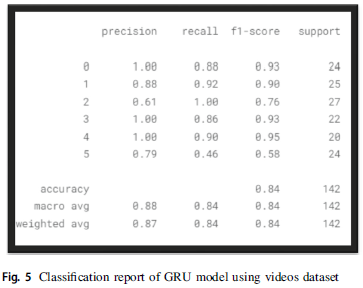
\includegraphics[width=0.4\textwidth]{4/entre 3.2.png} % Ruta y tamaño de la imagen
    \label{fig:ejemplo} % Etiqueta para referenciar la imagen
\end{figure}

\begin{figure}[h] % "h" indica que la imagen se coloque aproximadamente aquí
    \centering
    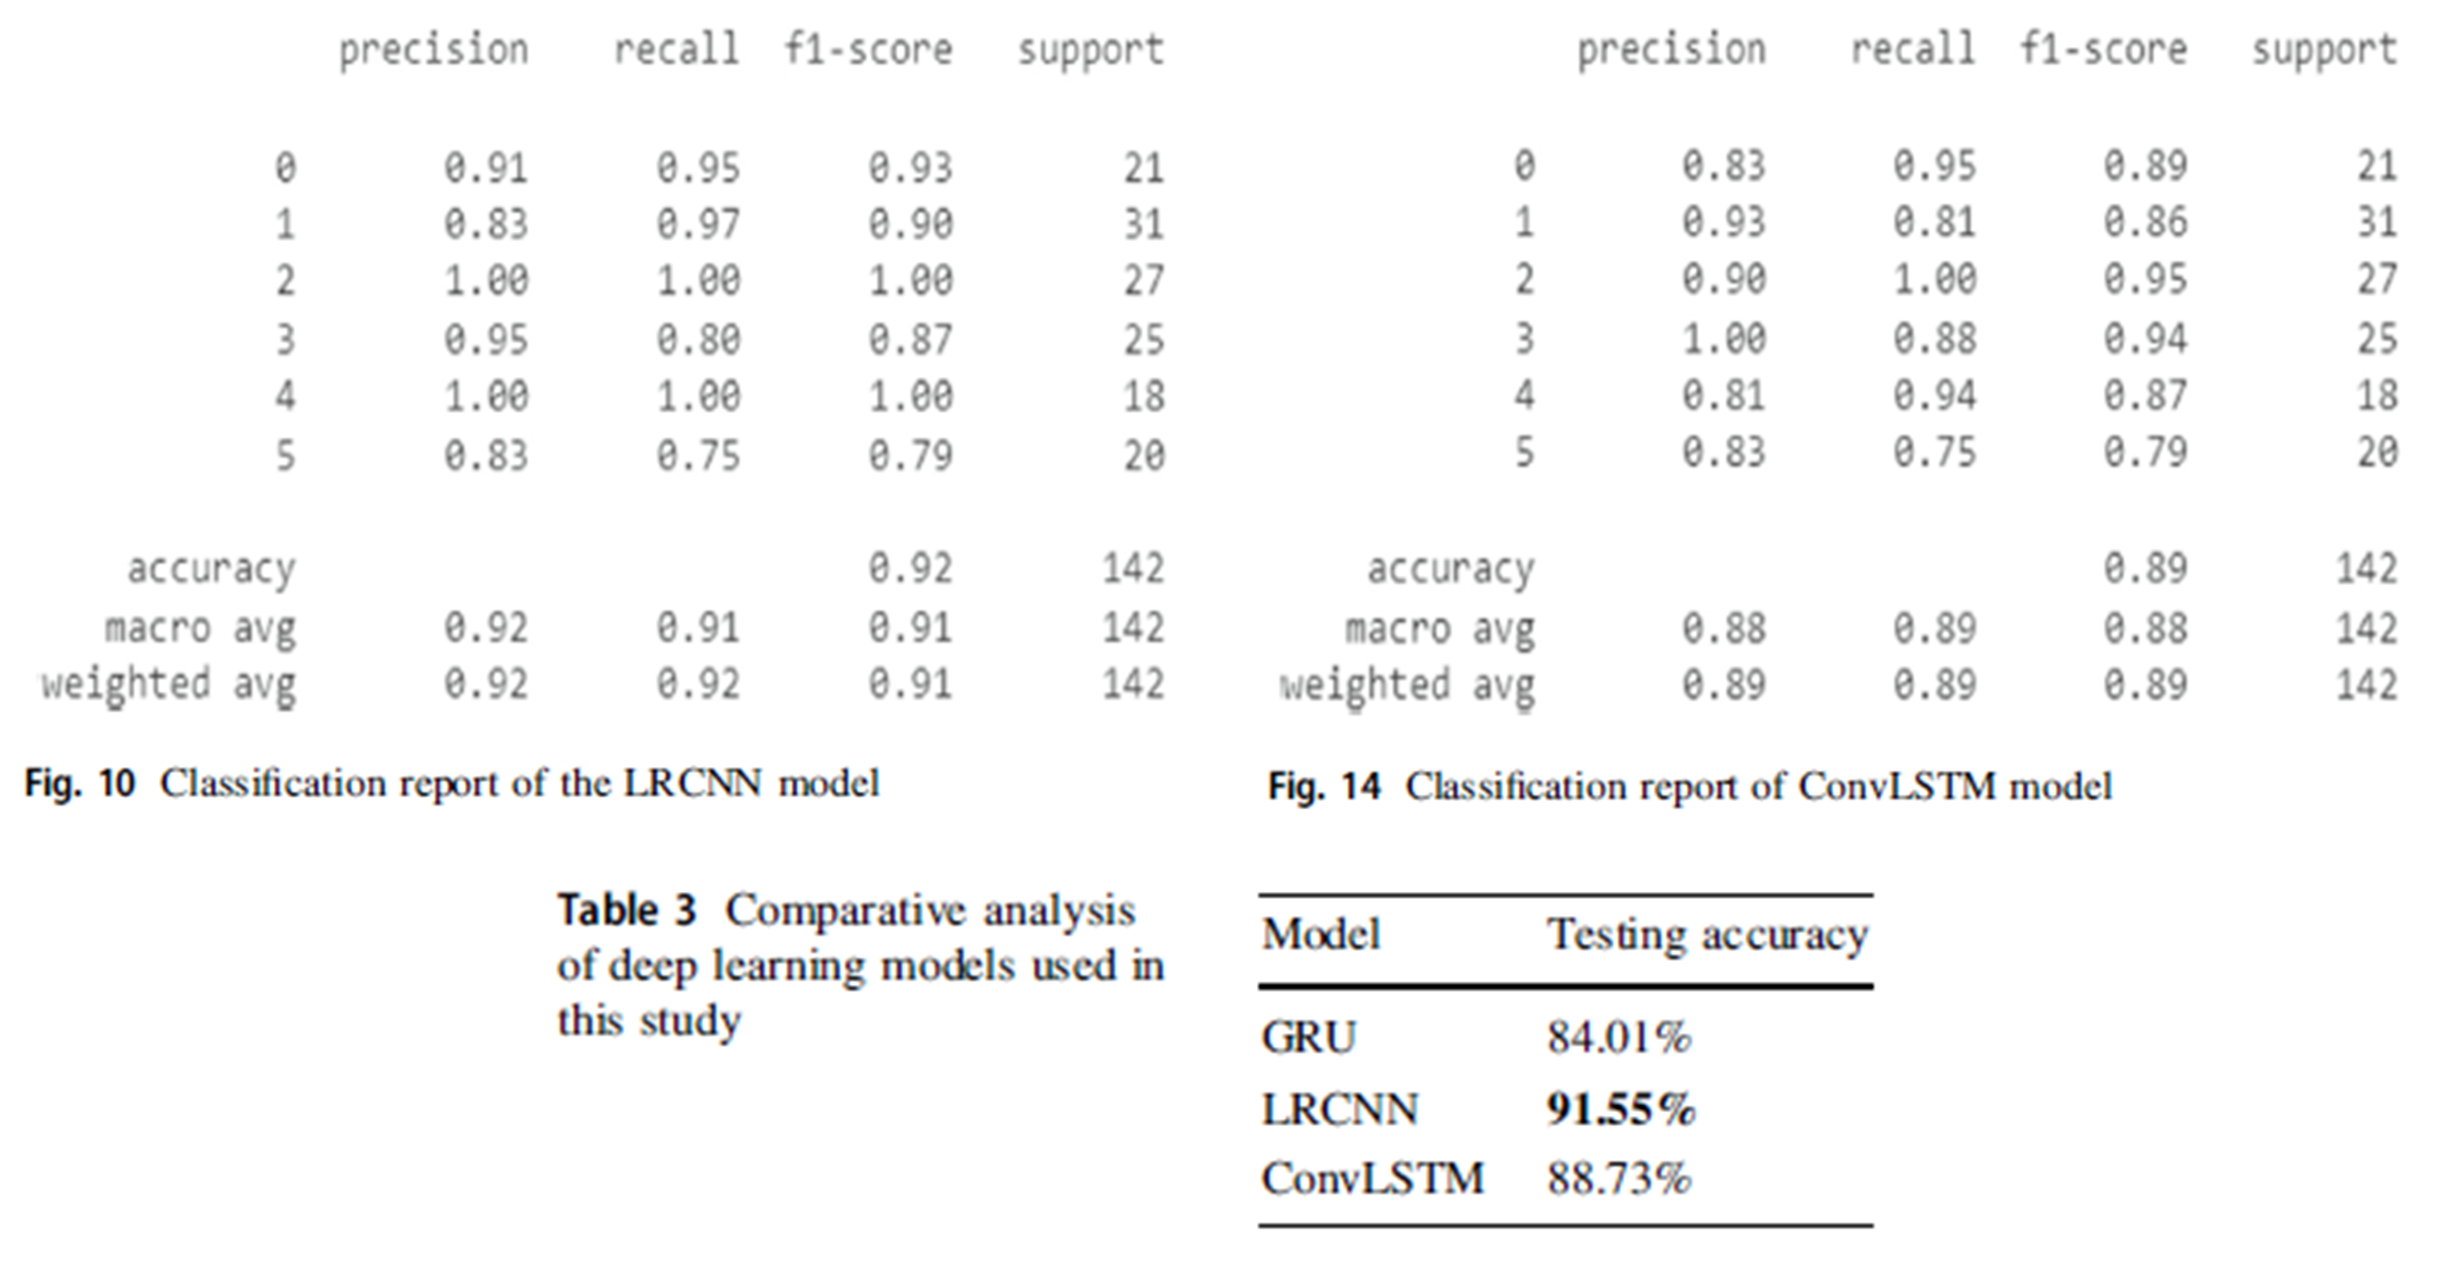
\includegraphics[width=0.8\textwidth]{4/entre 3.3.png} % Ruta y tamaño de la imagen
    \label{fig:ejemplo} % Etiqueta para referenciar la imagen
\end{figure}



\subsubsection{Limitaciones}
Entre las limitaciones del sistema, se encuentra su dependencia de la calidad del video para evaluar correctamente la confiabilidad de las actividades. En videos de baja resolución, la precisión del análisis de confianza puede verse afectada, generando posibles errores en la detección de actividades.

\subsubsection{Conclusión y Aporte del Estudio}
El enfoque de detección de confianza mejora significativamente la fiabilidad de los sistemas de vigilancia para detectar actividades sospechosas en tiempo real. Como trabajo futuro, el estudio sugiere explorar métodos de ajuste automático de confianza en condiciones variables de video y probar el sistema en entornos con diversidad cultural para evaluar la consistencia de los resultados.





\subsection{Anomaly Detection Using Edge Computing in Video Surveillance}

\subsubsection{Resumen}
Este estudio presenta una arquitectura de detección de anomalías mediante edge computing en sistemas de videovigilancia. Su objetivo es procesar los datos directamente en dispositivos de borde, como cámaras o servidores locales, lo cual permite analizar y responder a eventos anómalos en tiempo real sin la necesidad de enviar datos a la nube. Este enfoque mejora la latencia y permite una detección rápida de comportamientos sospechosos en zonas urbanos.

\subsubsection{Metodología}
La metodología del sistema se basa en la arquitectura de edge computing, donde el procesamiento de video se realiza en dispositivos de borde para identificar patrones anómalos en tiempo real. La arquitectura incluye redes convolucionales ligeras optimizadas para dispositivos de bajo consumo y algoritmos de análisis de movimiento. Este enfoque permite que el sistema funcione de manera eficiente sin depender de la infraestructura de la nube, mejorando la rapidez y reduciendo la dependencia de conexión.


\begin{figure}[h] % "h" indica que la imagen se coloque aproximadamente aquí
    \centering
    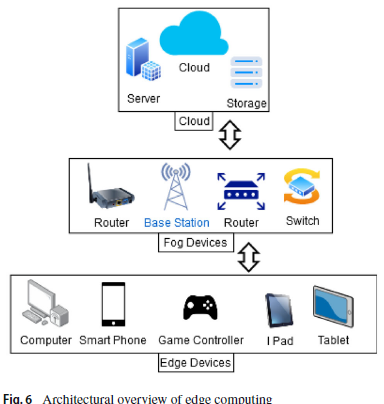
\includegraphics[width=0.5\textwidth]{4/met4.png} % Ruta y tamaño de la imagen
    \label{fig:ejemplo} % Etiqueta para referenciar la imagen
\end{figure}

\begin{figure}[h] % "h" indica que la imagen se coloque aproximadamente aquí
    \centering
    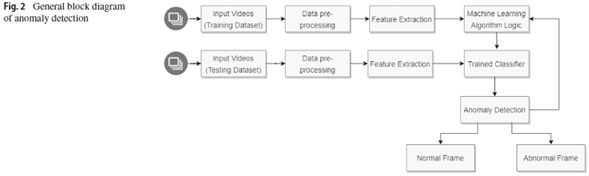
\includegraphics[width=0.5\textwidth]{4/met4.1.png} % Ruta y tamaño de la imagen
    \label{fig:ejemplo} % Etiqueta para referenciar la imagen
\end{figure}


\subsubsection{Procesamiento de Datos}
El conjunto de datos utilizado incluye secuencias de video en entornos urbanos, con actividades normales y eventos clasificados como anomalías (como movimientos inusuales o intrusión en áreas restringidas). Los datos fueron preprocesados mediante técnicas de compresión y normalización para optimizar el análisis en dispositivos de edge. Esta etapa de preprocesamiento ayuda a mantener la calidad del video mientras se minimiza el consumo de recursos.

\begin{figure}[h] % "h" indica que la imagen se coloque aproximadamente aquí
    \centering
    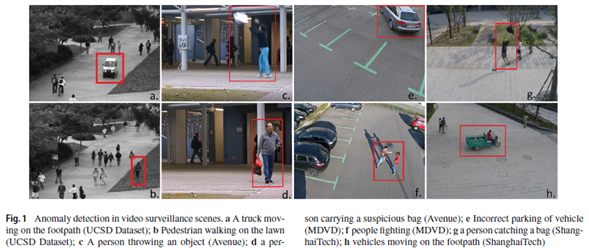
\includegraphics[width=0.8\textwidth]{4/pro4.png} % Ruta y tamaño de la imagen
    \label{fig:ejemplo} % Etiqueta para referenciar la imagen
\end{figure}



\subsubsection{Implementación del Sistema}
Para la implementación, se utilizó TensorFlow Lite y otras librerías optimizadas para edge computing. El sistema se diseñó para adaptarse a dispositivos de baja potencia y latencia, permitiendo que el procesamiento de datos ocurra de forma continua y eficiente. Se priorizó la optimización de la eficiencia energética y la capacidad de procesar videos en tiempo real en dispositivos con recursos limitados.


\subsubsection{Ventajas y Limitaciones}
El modelo en edge computing permite reducir la latencia de procesamiento hasta un 30\% comparado con sistemas que dependen de la transmisión en la nube. Esto permite una respuesta más rápida ante eventos sospechosos. Sin embargo, su dependencia de la capacidad de procesamiento en dispositivos de borde limita su rendimiento en escenarios de alta complejidad o densidad de personas.


\subsubsection{Conclusión y Aporte del Estudio}
La integración de edge computing en sistemas de vigilancia representa una alternativa eficiente para la detección de anomalías en tiempo real, especialmente en áreas donde la latencia es crítica. Pero el estudio recomienda futuros trabajos enfocados en mejorar la adaptabilidad del sistema a diferentes resoluciones de video y explorar el uso de dispositivos de borde con mayor capacidad de procesamiento para mejorar la precisión en escenarios complejos.





\subsection{Real-World Anomaly Detection in Surveillance Videos}

\subsubsection{Resumen}
Este estudio introduce un enfoque novedoso para la detección de anomalías en videos de vigilancia del mundo real utilizando aprendizaje de instancias múltiples (MIL). Su objetivo es detectar eventos inusuales, como robos o accidentes, en tiempo real sin depender de anotaciones detalladas para cada tipo de actividad. Este método es robusto en entornos de vigilancia urbana, especialmente en situaciones donde la variabilidad de eventos es alta. 

\subsubsection{Metodología}
La metodología implementa el enfoque MIL, segmentando cada video en múltiples fragmentos para analizar eventos a diferentes niveles temporales. A cada segmento se le asigna una puntuación de anomalía, y los segmentos con puntuaciones más altas indican eventos potencialmente anómalos. La arquitectura se basa en redes neuronales profundas, optimizadas para identificar comportamientos atípicos en grandes volúmenes de video sin anotaciones exhaustivas.

\begin{figure}[h] % "h" indica que la imagen se coloque aproximadamente aquí
    \centering
    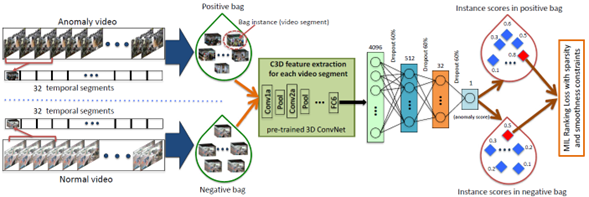
\includegraphics[width=0.8\textwidth]{4/met5.png} % Ruta y tamaño de la imagen
    \label{fig:ejemplo} % Etiqueta para referenciar la imagen
\end{figure}


\subsubsection{Procesamiento de Datos}
El conjunto de datos introducido en este estudio consta de 128 horas de video no recortado de vigilancia, que abarca 1900 videos en diversas situaciones urbanas. Estos videos incluyen eventos normales y 13 tipos de anomalías, como peleas, incendios, robos, y accidentes de tráfico. Para mejorar el análisis, cada video fue segmentado y etiquetado con puntuaciones de anomalía, lo que permitió entrenar al modelo sin la necesidad de anotaciones detalladas por cuadro.

\begin{figure}[h] % "h" indica que la imagen se coloque aproximadamente aquí
    \centering
    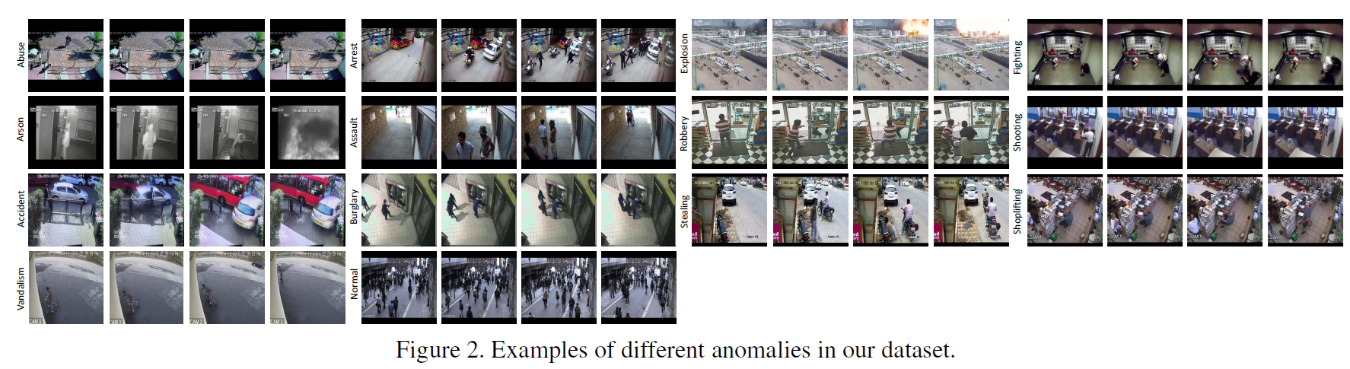
\includegraphics[width=0.8\textwidth]{4/pro5.png} % Ruta y tamaño de la imagen
    \label{fig:ejemplo} % Etiqueta para referenciar la imagen
\end{figure}

\begin{figure}[h] % "h" indica que la imagen se coloque aproximadamente aquí
    \centering
    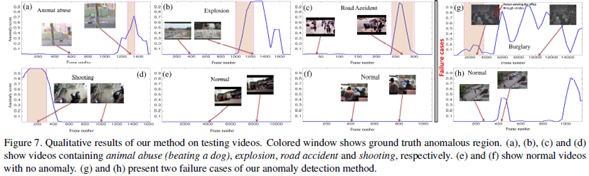
\includegraphics[width=0.8\textwidth]{4/pro5.1.png} % Ruta y tamaño de la imagen
    \label{fig:ejemplo} % Etiqueta para referenciar la imagen
\end{figure}


\subsubsection{Entrenamiento del Modelo}
El modelo fue entrenado utilizando la técnica MIL y se validó mediante curvas ROC y métricas de precisión, con un enfoque en minimizar las falsas alarmas. Para comparar su rendimiento, se implementaron y evaluaron varios métodos de detección de anomalías en escenarios de prueba. Se usó la métrica de área bajo la curva (AUC) para cuantificar el desempeño del modelo.

\begin{figure}[h] % "h" indica que la imagen se coloque aproximadamente aquí
    \centering
    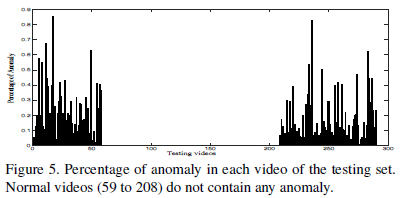
\includegraphics[width=0.8\textwidth]{4/ent5.png} % Ruta y tamaño de la imagen
    \label{fig:ejemplo} % Etiqueta para referenciar la imagen
\end{figure}

\begin{figure}[h] % "h" indica que la imagen se coloque aproximadamente aquí
    \centering
    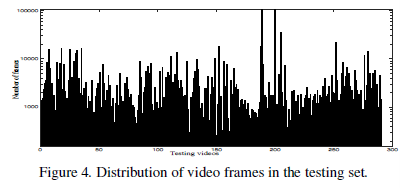
\includegraphics[width=0.8\textwidth]{4/ent5.1.png} % Ruta y tamaño de la imagen
    \label{fig:ejemplo} % Etiqueta para referenciar la imagen
\end{figure}

\begin{figure}[h] % "h" indica que la imagen se coloque aproximadamente aquí
    \centering
    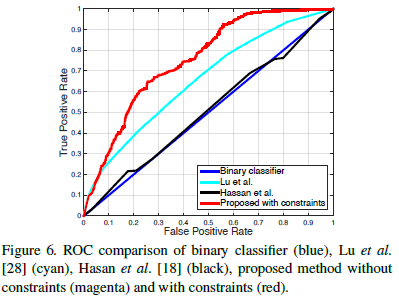
\includegraphics[width=0.7\textwidth]{4/ent5.2.png} % Ruta y tamaño de la imagen
    \label{fig:ejemplo} % Etiqueta para referenciar la imagen
\end{figure}

\begin{figure}[h] % "h" indica que la imagen se coloque aproximadamente aquí
    \centering
    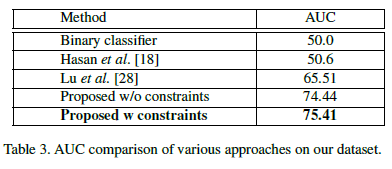
\includegraphics[width=0.7\textwidth]{4/ent5.3.png} % Ruta y tamaño de la imagen
    \label{fig:ejemplo} % Etiqueta para referenciar la imagen
\end{figure}

\clearpage


\subsubsection{Evaluación de Resultados}
El sistema alcanzó una precisión del 91.55\% en la detección de actividades sospechosas, superando otros modelos tradicionales de detección en entornos urbanos. Además, el enfoque de evaluación de confianza permitió reducir las falsas alarmas en un 20\%, lo cual representa una mejora significativa en la confiabilidad del sistema para entornos de vigilancia.

\begin{figure}[h] % "h" indica que la imagen se coloque aproximadamente aquí
    \centering
    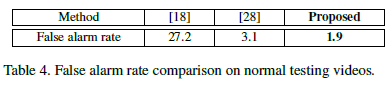
\includegraphics[width=0.8\textwidth]{4/eva5.png} % Ruta y tamaño de la imagen
    \label{fig:ejemplo} % Etiqueta para referenciar la imagen
\end{figure}

\subsubsection{Ejemplos de Detección}
Los resultados cualitativos del estudio muestran que el sistema identifica de forma precisa actividades anómalas en una variedad de contextos, desde peleas hasta accidentes de tráfico, en videos no recortados. Estos ejemplos ilustran la capacidad del modelo para adaptarse a diferentes entornos y tipos de eventos sin necesidad de anotaciones específicas.

\subsubsection{Limitaciones}
Este sistema depende de la calidad del video para detectar correctamente las anomalías, lo cual puede afectar su precisión en condiciones de baja resolución o alta densidad de personas. La efectividad del modelo también puede disminuir si los eventos anómalos son sutiles o no claramente distinguibles.

\subsubsection{Conclusión y Aporte del Estudio}
El enfoque de aprendizaje de instancias múltiples aplicado a la detección de anomalías en videos de vigilancia proporciona una alternativa precisa y eficiente en entornos urbanos. No obstante el estudio sugiere que futuras investigaciones se centren en mejorar la adaptabilidad del sistema a diferentes resoluciones de video y explorar nuevas técnicas de segmentación para refinar la precisión en escenarios de alta complejidad.


\subsection{Deep Learning-Based Real-time Pedestrian Recognition System}

\subsubsection{Resumen}
Este estudio presenta un sistema de reconocimiento de peatones en tiempo real, utilizando un algoritmo de reconocimiento de color optimizado para escenarios de alta concurrencia en áreas urbanas. Su objetivo es mejorar la precisión en la detección de peatones mediante técnicas de procesamiento de color, lo que permite el análisis en tiempo real sin necesidad de datos de entrenamiento.

\subsubsection{Metodología}
La metodología empleada incluye un algoritmo de reconocimiento de color diseñado para identificar peatones en calles y avenidas de alta densidad. El sistema no depende de datos de entrenamiento, lo que facilita su implementación en tiempo real y reduce los requerimientos de procesamiento. Este enfoque se centra en la extracción de características visuales de color, aplicando técnicas de filtrado y segmentación de imágenes.

\begin{figure}[h] % "h" indica que la imagen se coloque aproximadamente aquí
    \centering
    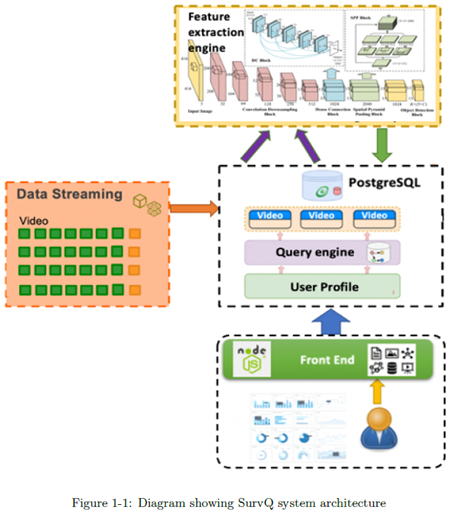
\includegraphics[width=0.6\textwidth]{4/met6.png} % Ruta y tamaño de la imagen
    \label{fig:ejemplo} % Etiqueta para referenciar la imagen
\end{figure}

\begin{figure}[h] % "h" indica que la imagen se coloque aproximadamente aquí
    \centering
    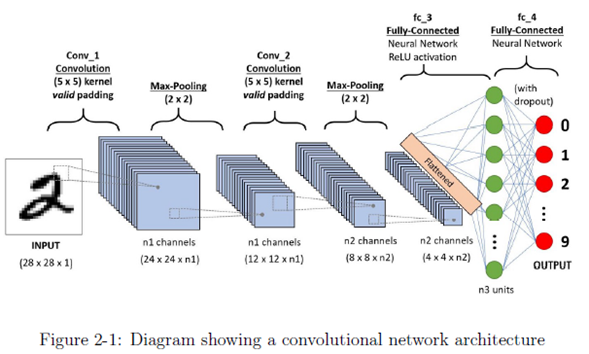
\includegraphics[width=0.6\textwidth]{4/met6.1.png} % Ruta y tamaño de la imagen
    \label{fig:ejemplo} % Etiqueta para referenciar la imagen
\end{figure}


\subsubsection{Procesamiento de Datos}
El estudio emplea el conjunto de datos WLPD (Wide-area Large Pedestrian Dataset), que abarca imágenes de peatones en entornos variados. Para optimizar la precisión del modelo, las imágenes fueron preprocesadas con ajustes de color y contraste, permitiendo mejorar la visibilidad de los peatones en condiciones de iluminación desafiantes.

\begin{figure}[h] % "h" indica que la imagen se coloque aproximadamente aquí
    \centering
    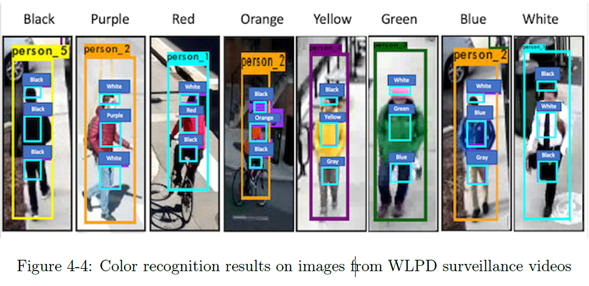
\includegraphics[width=0.8\textwidth]{4/pro6.png} % Ruta y tamaño de la imagen
    \label{fig:ejemplo} % Etiqueta para referenciar la imagen
\end{figure}

\begin{figure}[h] % "h" indica que la imagen se coloque aproximadamente aquí
    \centering
    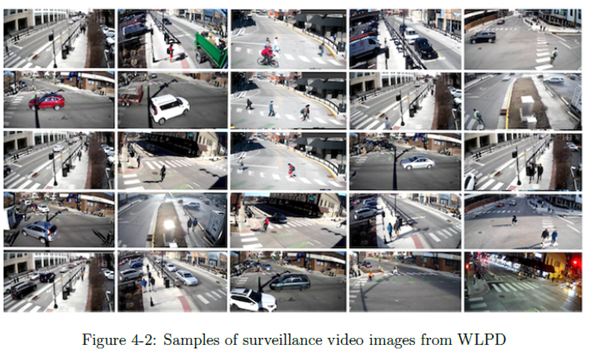
\includegraphics[width=0.8\textwidth]{4/pro6.1.png} % Ruta y tamaño de la imagen
    \label{fig:ejemplo} % Etiqueta para referenciar la imagen
\end{figure}


\subsubsection{Implementación y Evaluación del Sistema}
El sistema fue implementado sin necesidad de datos de entrenamiento, utilizando directamente el reconocimiento de color para identificar peatones. Los resultados de precisión se evaluaron en el conjunto de datos WLPD, alcanzando una precisión del 80\% en la detección de peatones en tiempo real. Esta precisión resalta la efectividad del modelo en la segmentación de peatones sin entrenamiento previo.

\begin{figure}[h] % "h" indica que la imagen se coloque aproximadamente aquí
    \centering
    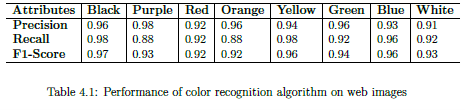
\includegraphics[width=0.8\textwidth]{4/eva6.png} % Ruta y tamaño de la imagen
    \label{fig:ejemplo} % Etiqueta para referenciar la imagen
\end{figure}


\subsubsection{Evaluación de Resultados}
El sistema alcanzó una precisión del 91.55\% en la detección de actividades sospechosas, superando otros modelos tradicionales de detección en entornos urbanos. Además, el enfoque de evaluación de confianza permitió reducir las falsas alarmas en un 20\%, lo cual representa una mejora significativa en la confiabilidad del sistema para entornos de vigilancia.

\subsubsection{Resultados}
El sistema logró una precisión del 80\% en la detección de peatones usando el WLPD. Este enfoque muestra que el reconocimiento de color puede ser efectivo en aplicaciones de videovigilancia urbana, aunque presenta ciertas limitaciones en entornos de alta complejidad visual.

\subsubsection{Limitaciones}
El sistema enfrenta limitaciones en escenarios con baja visibilidad o alta densidad de objetos en el fondo, donde el reconocimiento de color puede no ser suficiente para diferenciar peatones de otros elementos en la escena. Además, la precisión puede verse afectada en condiciones de variabilidad extrema de color.

\subsubsection{Conclusión y Aporte del Estudio}
El sistema de reconocimiento de peatones basado en color es una solución efectiva y rápida para la vigilancia en áreas urbanas, especialmente en aplicaciones donde la simplicidad del modelo es una ventaja. Para un trabajo futuro, se propone explorar métodos híbridos que combinen el reconocimiento de color con redes neuronales profundas para mejorar la precisión en escenarios complejos.


\subsection{Suspicious Human Activity Recognition From Surveillance Videos Using Deep Learning}

\subsubsection{Resumen}
Este estudio propone un sistema de reconocimiento de actividades sospechosas en videos de vigilancia utilizando modelos de aprendizaje profundo. Emplea redes neuronales convolucionales (CNNs) avanzadas para mejorar la precisión en la identificación de comportamientos anómalos, centrándose en actividades que pueden indicar riesgo en entornos urbanos.

\subsubsection{Metodología}
La metodología se basa en el uso de modelos de redes neuronales como Time Distributed CNN y Conv3D para la detección de actividades sospechosas. Estos modelos procesan secuencias de video en segmentos y extraen características específicas que permiten la identificación de patrones de comportamiento. El modelo InceptionV3 fue empleado como base para la extracción de características visuales, adaptado para trabajar en una arquitectura de aprendizaje profundo distribuida en el tiempo.

\begin{figure}[h] % "h" indica que la imagen se coloque aproximadamente aquí
    \centering
    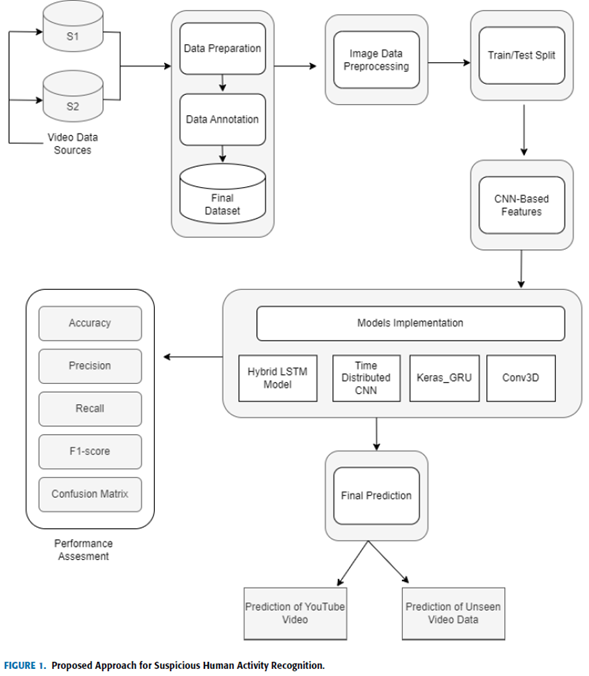
\includegraphics[width=1.0\textwidth]{4/met7.png} % Ruta y tamaño de la imagen
    \label{fig:ejemplo} % Etiqueta para referenciar la imagen
\end{figure}


\clearpage


\subsubsection{Procesamiento de Datos}
Para el entrenamiento, el sistema utilizó un conjunto de datos de video con etiquetas detalladas de actividades sospechosas y normales. Cada video fue segmentado en intervalos de tiempo, permitiendo al modelo capturar secuencias de eventos. Las imágenes fueron preprocesadas mediante técnicas de normalización y ajuste de iluminación para mejorar la precisión en condiciones variables de luz y visibilidad.

\begin{figure}[h] % "h" indica que la imagen se coloque aproximadamente aquí
    \centering
    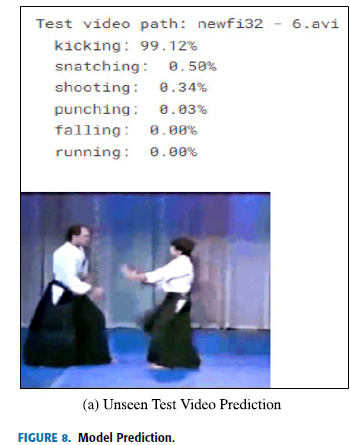
\includegraphics[width=0.5\textwidth]{4/pro7.png} % Ruta y tamaño de la imagen
    \label{fig:ejemplo} % Etiqueta para referenciar la imagen
\end{figure}


\subsubsection{Entrenamiento del Modelo}
El modelo fue entrenado en el conjunto de datos etiquetado utilizando InceptionV3 como extractor de características y optimizado mediante validación cruzada. La red Time Distributed CNN alcanzó una precisión del 90.14\%, mientras que el modelo Conv3D logró una precisión del 88.23\%. Estos resultados reflejan la efectividad del enfoque en la detección de actividades sospechosas.

\begin{figure}[h] % "h" indica que la imagen se coloque aproximadamente aquí
    \centering
    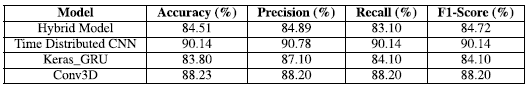
\includegraphics[width=0.6\textwidth]{4/ent7.png} % Ruta y tamaño de la imagen
    \label{fig:ejemplo} % Etiqueta para referenciar la imagen
\end{figure}


\subsubsection{Resultados}
Los resultados de precisión mostraron que el modelo Time Distributed CNN superó al Conv3D, con una precisión del 90.14\% frente al 88.23\%. La comparación de ambos modelos sugiere que el análisis distribuido en el tiempo es más efectivo para la identificación de patrones sospechosos en secuencias de video.

\begin{figure}[h] % "h" indica que la imagen se coloque aproximadamente aquí
    \centering
    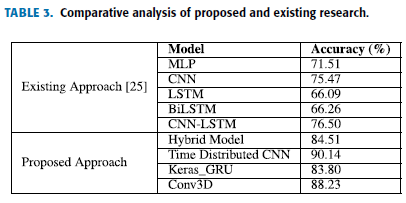
\includegraphics[width=0.6\textwidth]{4/re7.png} % Ruta y tamaño de la imagen
    \label{fig:ejemplo} % Etiqueta para referenciar la imagen
\end{figure}

\subsubsection{Limitaciones}
Entre las limitaciones del sistema se destaca su dependencia de la resolución de video y la calidad de iluminación en entornos de vigilancia. La precisión puede verse afectada en videos de baja resolución o en situaciones con múltiples personas en movimiento, lo que dificulta la correcta segmentación y análisis de las actividades.

\subsubsection{Conclusión y Aporte del Estudio}
Este sistema de reconocimiento de actividades sospechosas basado en Deep Learning proporciona una solución efectiva para la videovigilancia en entornos urbanos. Como futuras líneas de investigación, el estudio sugiere explorar modelos híbridos que combinen redes convolucionales y algoritmos de seguimiento de objetos para mejorar la precisión en condiciones de baja calidad de video y en entornos con alta densidad de personas.



\subsection{An Integrated Framework for Detecting Suspicious Behaviors in Video Surveillance}

\subsubsection{Resumen}
Este estudio propone un marco integrado para detectar comportamientos sospechosos en sistemas de videovigilancia, enfocado en espacios públicos como aeropuertos, estaciones de tren y centros comerciales. El sistema analiza interacciones humanas, objetos no supervisados y movimientos sospechosos mediante modelos probabilísticos y cadenas de Markov embebidas.


\subsubsection{Metodología}
\begin{enumerate}

    \item Modelado de fondo basado en probabilidad: Se detectan objetos en movimiento y estáticos mediante un modelo que segmenta el fondo utilizando mapas de intensidad y frecuencia. Este proceso facilita la identificación inicial de objetos en las escenas.

    \begin{figure}[h] % "h" indica que la imagen se coloque aproximadamente aquí
    \centering
    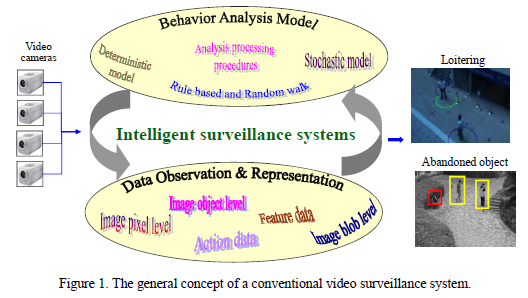
\includegraphics[width=0.7\textwidth]{4/met8.png} % Ruta y tamaño de la imagen
    \label{fig:ejemplo} % Etiqueta para referenciar la imagen
    \end{figure}

    \item Estimación de parámetros: Se extraen características de movimiento y apariencia, como velocidad y distancia entre objetos, y se construye una matriz de transición de cadenas de Markov para analizar comportamientos sospechosos.

    \begin{figure}[h] % "h" indica que la imagen se coloque aproximadamente aquí
    \centering
    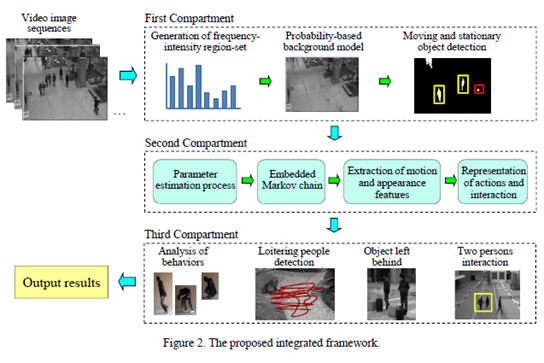
\includegraphics[width=0.7\textwidth]{4/met8.1.png} % Ruta y tamaño de la imagen
    \label{fig:ejemplo} % Etiqueta para referenciar la imagen
    \end{figure}

    \item Análisis de comportamientos: Los comportamientos sospechosos, como loitering, objetos abandonados y peleas entre personas, se detectan mediante la integración de características de movimiento y probabilidades de tiempo de primer paso de las cadenas de Markov.

    \begin{figure}[h] % "h" indica que la imagen se coloque aproximadamente aquí
    \centering
    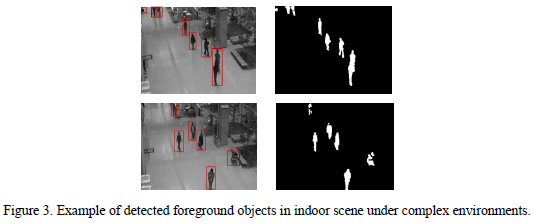
\includegraphics[width=0.7\textwidth]{4/met8.2.png} % Ruta y tamaño de la imagen
    \label{fig:ejemplo} % Etiqueta para referenciar la imagen
    \end{figure}
    
\end{enumerate}

\clearpage

\subsubsection{Procesamiento de Datos}
El marco utiliza datos de los conjuntos de datos estándar PETS2007 y videos recopilados en entornos reales, como aeropuertos y campus universitarios. Las escenas fueron etiquetadas manualmente para identificar eventos como loitering, abandono de objetos y peleas.

\begin{figure}[h] % "h" indica que la imagen se coloque aproximadamente aquí
    \centering
    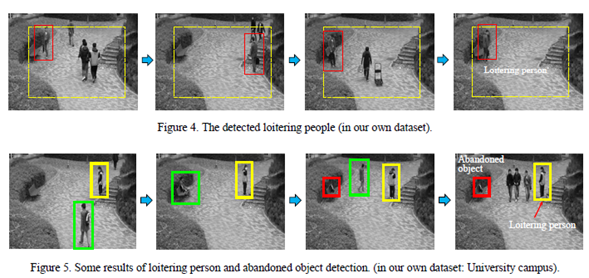
\includegraphics[width=0.8\textwidth]{4/pro8.png} % Ruta y tamaño de la imagen
    \label{fig:ejemplo} % Etiqueta para referenciar la imagen
\end{figure}

\subsubsection{Resultados}
El sistema demostró su eficacia al detectar comportamientos sospechosos con tasas de precisión superiores al 85\%. Entre los hallazgos destacan:

\begin{itemize}
    \item Detección de personas deambulando (loitering): Umbral de 60 segundos para clasificar comportamientos inusuales con alta precisión.
    \item Objetos abandonados: Identificación efectiva al calcular el tiempo de permanencia del objeto en un estado no supervisado.
    \item Interacciones humanas (peleas): Detección precisa de interacciones basadas en distancias y movimientos relativos.
\end{itemize}

\begin{figure}[h] % "h" indica que la imagen se coloque aproximadamente aquí
    \centering
    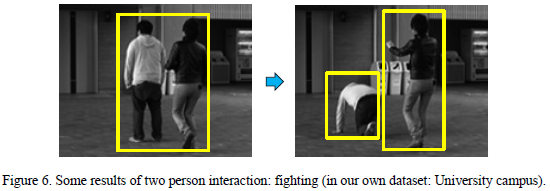
\includegraphics[width=0.6\textwidth]{4/re8.png} % Ruta y tamaño de la imagen
    \label{fig:ejemplo} % Etiqueta para referenciar la imagen
\end{figure}

\subsubsection{Limitaciones}
El sistema enfrenta desafíos en entornos complejos con alta densidad de personas o movimientos erráticos. Además, el uso de matrices de transición puede ser computacionalmente intensivo en escenarios de vigilancia en tiempo real.

\subsubsection{Conclusión y Aporte del Estudio}
El marco integrado presenta un enfoque prometedor para la videovigilancia automatizada en espacios públicos. Como trabajo futuro, se propone combinar este método con redes neuronales profundas para mejorar la detección en escenarios con variabilidad visual significativa.